\chapter{Introduction}
\label{1}
\section{Motivation}

With the development of science and technology, there may arise crucial 
problems. Rising traffic in the country gives birth to rising accidents. To 
avoid/minimize the accidents, proper surveillance is required. Detection 
and tracking of vehicles have become a key component in traffic 
surveillance and automatic driving. Traditional algorithms like Gaussian 
Mixed Model (GMM) has achieved encouraging success in this field \cite{chap_1_article:1}. But due 
to variation in illumination, occlusion, background clutter etc. detection 
of vehicles is still a challenge. 
Deep Neural Networks (DNNs) have gained a lot of attention in 
past few years. Due to the betterment of deep learning, object 
detection has achieved major advancements in recent years. The work 
in this project is based on DNNs to detect and classify vehicles from 
a dataset collected from images and videos.

\section{Background}

Classical methods of vehicle detection were based on some 
sort of features like symmetry, edges, texture, underbody shadows 
and corners \cite{chap_1_article:2}. These methods were easy to describe and perform 
in specific kind of applications. These methods fail in many situations 
like due to less illumination of highway. With the advent of 
deep learning, a subset of machine learning, the detection and 
classification mechanism have dramatically improved. Machine learning 
and deep learning are sub-branches of computer intelligence which help 
in the process of vehicle classification to event detection. 
Using deep learing techniques, we are going to focus on a specific kind 
of detection (deep learning has grown its branches in almost every 
kind of image recongnition, text recognition, face detection etc), vehicle 
detection. Using deep learning based Convolutional Neural Networks (CNNs) 
which is a wide field for object detection, classification, sementic 
segmenation etc. These networks take input images, learn features, adjust 
weights and then detect the targets from test data. In deep learning, 
algorithms automatically learn features unlike machine 
learning algorithms, we have to pass features to train the 
model. Our work is based on Deep Neural Networks (DNNs).

\section{Goals \& Objectives}

The goal of this project is to make a deep learning based model (using Python) for vehicle detection and classification. Main objectives are summarized as:
\begin{itemize}
\item Collection of datasets (images dataset of car, truck classes etc. and videos).
\item Design of Convolutional Neural Network
\item Configuration of training options (AlexNet, VGGNet, ResNet etc.)
\item Training of detector (RCNN, Fast- RCNN, Faster-RCNN, YOLO etc.)
\item Evaluation of the trained detector
\end{itemize}

\section{Challenges}

Human can understand and interpret images in a 
second or less. For machines, it is not easy to achieve 
accurate results unless models are trained properly. Firstly, proper 
training is a challenging task for a customized data. Detection 
algorithms are also hard to implement as we must have recommended 
GPU requirements and best choice of algorithm for good results. Videos 
which are moving frames, it is difficult to draw accurate bounding boxes 
in a video having say 30 frames per second 
means 30 images are splashed in a second. 	


\section{Organization of Thesis}

\textbf{Chapter \ref{Chapter 2}}: Chapter 2 is about literature review. It is about
the whole reading and understanding of Image classification \& detection.

\noindent\textbf{Chapter \ref{Chapter 3}}: This chapter is about Convolutional Neural Networks. All CNN architectures with their details
are discussed.



% \begin{figure}[H]
% 	\centering
% 	%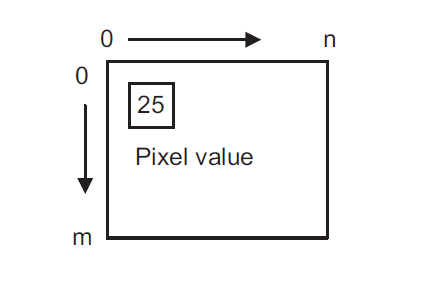
\includegraphics[scale = 0.5]{CHAPTERS/Chapter-2/Images/2.2.png}
% 	\caption{Grayscale Image format}
% 	\label{fig:1.1}
% \end{figure}